% DASHSys Workshop Paper: DataPup — Human-in-the-loop analytical Text-to-SQL
% Format: acmart sigconf
\documentclass[sigconf, nonacm]{acmart}

% PVLDB-specific settings
\AtBeginDocument{%
  \providecommand\BibTeX{{%
    Bib\TeX}}}

% Remove ACM-specific metadata
\settopmatter{printacmref=false}
\renewcommand\footnotetextcopyrightpermission[1]{}

% PVLDB/DASHSys review metadata. Page numbers are shown for review.
\newcommand\vldbdoi{XX.XX/XXX.XX}
\newcommand\vldbpages{XXX-XXX}
\newcommand\vldbvolume{19}
\newcommand\vldbissue{1}
\newcommand\vldbyear{2026}
\newcommand\vldbauthors{\authors}
\newcommand\vldbtitle{\shorttitle}
\newcommand\vldbavailabilityurl{https://github.com/DataPupOrg/DataPup-Research}
\newcommand\vldbpagestyle{plain}

\usepackage{graphicx}
\usepackage{booktabs}
\usepackage{multirow}
\usepackage{xcolor}
\usepackage{tikz}
\usetikzlibrary{positioning, arrows.meta, fit, backgrounds, shapes.geometric}

\graphicspath{{evaluation/results/figures/}}

\begin{document}

\title{DataPup: Schema-Aware and Execution-Aware Text-to-SQL for Human-in-the-Loop Analytical Database Clients}

\author{Sahith Vibudhi}
\affiliation{\institution{Independent Researcher}\city{San Francisco}\state{California}\country{USA}}
\email{v.sahithkumar@gmail.com}

\author{Krishna Chaitanya Balusu}
\affiliation{\institution{Independent Researcher}\city{San Francisco}\state{California}\country{USA}}
\email{krishnabkc15@gmail.com}

\begin{abstract}
DataPup is an open-source, AI-assisted database client that translates natural language queries into SQL for analytical databases including ClickHouse, PostgreSQL, and MySQL. Featured in the LangChain ecosystem and the official ClickHouse documentation, DataPup uses a LangChain-based agent with seven schema discovery tools to iteratively introspect database structure and generate SQL. A key challenge in production is how to present schema information to the LLM: the choice of format, scope, metadata, and examples affects query correctness and the quality of the human-in-the-loop database experience. We study these prompt dimensions on three ClickHouse benchmarks (206 queries, 10 tables) with two Claude models, then validate with Claude, Codex, and Gemini CLI runs plus a focused DuckDB experiment. On the 150-query custom analytics benchmark, DataPup's current full-schema JSON style achieves only 17.3\% result correctness, while the revised prompt configuration reaches 66.0\% (McNemar exact $p{=}2.7{\times}10^{-19}$). Compared with a stronger full-schema zero-shot Markdown baseline, the revised configuration reaches 66.0\% versus 55.3\% RC in a planned paired comparison ($p{=}0.015$ raw; $p{=}0.075$ Holm-corrected). A leakage audit confirms that the few-shot pool is separate from the evaluation set; removing three near-duplicate flagged queries leaves best-configuration RC unchanged at 66.0\% on the remaining 147 queries. In the black-box CLI setting, the best configuration remains strongest for all three providers after one execution-repair attempt, reaching 56.0\% RC for Claude, 50.7\% for Codex, and 53.3\% for Gemini. On a focused DuckDB validation over 130 portable queries, the revised prompt matches the full-schema JSON baseline at 60.8\% RC while reaching 100.0\% execution success. The results motivate a DataPup production design that combines compact schema presentation, audited example retrieval, execution-aware repair, and explicit surfacing of remaining semantic assumptions to analysts.
\end{abstract}

\keywords{Text-to-SQL, Large Language Models, Prompt Engineering, Schema Linking, ClickHouse, OLAP, AI-Assisted Database Client}

\maketitle

%%% PVLDB block start %%%
\pagestyle{\vldbpagestyle}
\begingroup\small\noindent\raggedright\textbf{PVLDB Reference Format:}\\
\vldbauthors. \vldbtitle. PVLDB, \vldbvolume(\vldbissue): \vldbpages, \vldbyear.\\
\href{https://doi.org/\vldbdoi}{doi:\vldbdoi}
\endgroup
\begingroup
\renewcommand\thefootnote{}\footnote{\noindent
This work is licensed under the Creative Commons BY-NC-ND 4.0 International License. Visit \url{https://creativecommons.org/licenses/by-nc-nd/4.0/} to view a copy of this license. For any use beyond those covered by this license, obtain permission by emailing \href{mailto:info@vldb.org}{info@vldb.org}. Copyright is held by the owner/author(s). Publication rights licensed to the VLDB Endowment. \\
\raggedright Proceedings of the VLDB Endowment, Vol. \vldbvolume, No. \vldbissue\ %
ISSN 2150-8097. \\
\href{https://doi.org/\vldbdoi}{doi:\vldbdoi} \\
}\addtocounter{footnote}{-1}\endgroup

\ifdefempty{\vldbavailabilityurl}{}{
\begingroup\small\noindent\raggedright\textbf{PVLDB Artifact Availability:}\\
The source code, data, and experimental artifacts are available at \url{\vldbavailabilityurl}.
\endgroup
}
%%% PVLDB block end %%%

%% ====================================================================
\section{Introduction}
\label{sec:intro}

AI-assisted database clients are becoming essential tools for data analysts, enabling natural language interaction with complex database systems. DataPup is an open-source, cross-platform database client that uses LLM-based agents to help analysts explore and query analytical databases through natural language. In building and deploying DataPup, we encountered a fundamental design question: \emph{how should database schema information be presented to the LLM to maximize SQL generation accuracy?}

This question is critical for analytical databases (OLAP) like ClickHouse, DuckDB, and Snowflake, which present distinct challenges compared to the transactional databases (OLTP) that dominate existing Text-to-SQL benchmarks~\cite{yu2018spider}. OLAP systems feature columnar storage optimized for aggregation queries, specialized functions for time-series analysis, SQL dialect variations, and production schemas with hundreds of columns---all of which generic prompting strategies fail to capture.

Despite recent progress in LLM-based Text-to-SQL, with frontier models achieving execution accuracy exceeding 85\% on Spider~\cite{yu2018spider}, the impact of schema presentation on SQL generation remains underexplored. When a user asks ``Show me the top 10 customers by revenue last month,'' the LLM must understand which tables exist, what columns are available, their data types, relationships, and database-specific syntax. The effectiveness of SQL generation depends heavily on how this schema information is communicated---yet DataPup's production system naively includes all tables in raw JSON format, a strategy we found to be suboptimal.

In this paper, we present a systematic ablation study of schema-aware prompt engineering for Text-to-SQL targeting ClickHouse, investigating four dimensions of prompt design---schema format, scope, metadata enrichment, and example selection---across three benchmarks and two models. The findings directly inform DataPup's production schema presentation strategy, closing the loop between controlled experimentation and deployed system improvement.

Our contributions include:
\begin{itemize}
    \item The design and deployment of DataPup, an open-source AI-assisted database client with a LangChain-based agent architecture for natural language querying of analytical databases.
    \item A four-dimensional ablation analysis of schema format, scope, metadata, and example selection, with paired significance tests, a leakage audit for example retrieval, and a direct comparison against DataPup's current full-schema JSON prompt style.
    \item A multi-benchmark evaluation spanning 206 queries across three datasets with distinct structural characteristics (wide single-table, normalized multi-table, star schema), with cross-model validation on Claude 3.5 Sonnet and Claude Sonnet 4.
    \item A production-style CLI validation across Claude, Codex, and Gemini command-line agents, plus a focused DuckDB validation, including execution scoring and targeted SQL repair.
    \item Actionable guidelines for practitioners building AI-assisted database tools, with open-source release of our benchmark and evaluation framework.
\end{itemize}

%% ====================================================================
\section{System Overview: DataPup}
\label{sec:system}

DataPup\footnote{\url{https://github.com/DataPupOrg/DataPup}} is an open-source, cross-platform (macOS, Windows, Linux) AI-assisted database client that helps analysts explore and query analytical databases through natural language. The project is MIT-licensed with 294 GitHub stars and 41 forks as of early 2026, featured in the LangChain ecosystem and integrated into the official ClickHouse documentation as a recommended client. Built with Electron, React, and TypeScript, DataPup supports ClickHouse, PostgreSQL, and MySQL through a unified adapter layer. Figure~\ref{fig:architecture} provides an overview of the system architecture.

\begin{figure}[t]
\centering
\resizebox{\columnwidth}{!}{%
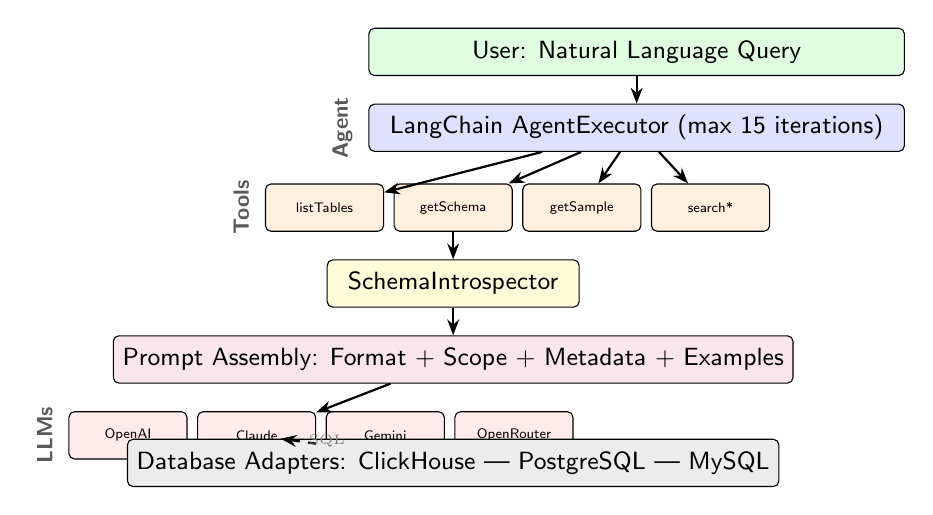
\begin{tikzpicture}[
    node distance=0.4cm and 0.3cm,
    box/.style={rectangle, draw, rounded corners=2pt, minimum height=0.6cm, font=\small\sffamily, align=center, fill=#1},
    box/.default=blue!8,
    arrow/.style={-{Stealth[length=2mm]}, thick},
    label/.style={font=\footnotesize\sffamily\bfseries, text=gray!70!black},
]
% User layer
\node[box=green!12, minimum width=6.8cm] (user) {User: Natural Language Query};

% Agent layer
\node[box=blue!12, minimum width=6.8cm, below=0.35cm of user] (agent) {LangChain AgentExecutor (max 15 iterations)};

% Tools row
\node[box=orange!12, below left=0.4cm and -0.2cm of agent, minimum width=1.5cm, font=\tiny\sffamily] (t1) {listTables};
\node[box=orange!12, right=0.12cm of t1, minimum width=1.5cm, font=\tiny\sffamily] (t2) {getSchema};
\node[box=orange!12, right=0.12cm of t2, minimum width=1.5cm, font=\tiny\sffamily] (t3) {getSample};
\node[box=orange!12, right=0.12cm of t3, minimum width=1.5cm, font=\tiny\sffamily] (t4) {search*};

% Schema introspector
\node[box=yellow!15, below=0.35cm of t2, minimum width=3.2cm] (schema) {SchemaIntrospector};

% Prompt assembly
\node[box=purple!10, below=0.35cm of schema, minimum width=6.8cm] (prompt) {Prompt Assembly: Format + Scope + Metadata + Examples};

% LLM Providers
\node[box=red!8, below left=0.35cm and -0.95cm of prompt, minimum width=1.5cm, font=\tiny\sffamily] (llm1) {OpenAI};
\node[box=red!8, right=0.12cm of llm1, minimum width=1.5cm, font=\tiny\sffamily] (llm2) {Claude};
\node[box=red!8, right=0.12cm of llm2, minimum width=1.5cm, font=\tiny\sffamily] (llm3) {Gemini};
\node[box=red!8, right=0.12cm of llm3, minimum width=1.5cm, font=\tiny\sffamily] (llm4) {OpenRouter};

% Database layer
\node[box=gray!15, below=0.7cm of prompt, minimum width=6.8cm] (db) {Database Adapters: ClickHouse | PostgreSQL | MySQL};

% Arrows
\draw[arrow] (user) -- (agent);
\draw[arrow] (agent) -- (t2);
\draw[arrow] (agent) -- (t1);
\draw[arrow] (agent) -- (t3);
\draw[arrow] (agent) -- (t4);
\draw[arrow] (t2) -- (schema);
\draw[arrow] (schema) -- (prompt);
\draw[arrow] (prompt) -- (llm2);
\draw[arrow, dashed] (llm2) -- node[right, font=\tiny, text=gray] {SQL} (db);

% Labels
\node[label, left=0.08cm of agent] {\rotatebox{90}{Agent}};
\node[label, left=0.08cm of t1] {\rotatebox{90}{Tools}};
\node[label, left=0.08cm of llm1] {\rotatebox{90}{LLMs}};

\end{tikzpicture}%
}
\caption{DataPup system architecture. The LangChain agent iteratively calls schema discovery tools, assembles prompts using the strategies evaluated in this paper, and routes to the user's selected LLM provider.}
\Description{Layered architecture diagram showing a user query flowing through a LangChain agent, schema discovery tools, prompt assembly, LLM providers, and database adapters.}
\label{fig:architecture}
\end{figure}

\subsection{Agent Architecture}
DataPup's natural language query pipeline is built on LangChain's agent framework. The core agent uses an \texttt{AgentExecutor} with tool-calling capabilities, supporting up to 15 iterative tool invocations per query. The system supports four LLM providers---OpenAI, Anthropic Claude, Google Gemini, and OpenRouter---enabling users to select their preferred model.

The agent has access to seven structured tools for schema discovery and query analysis:
\begin{enumerate}
    \item \texttt{listDatabases} --- enumerate available databases
    \item \texttt{listTables} --- retrieve tables within a database
    \item \texttt{getTableSchema} --- introspect column names, types, and constraints
    \item \texttt{getSampleRows} --- fetch sample data for context
    \item \texttt{searchTables} / \texttt{searchColumns} --- pattern-based schema search
    \item \texttt{analyzeQueryPerformance} --- EXPLAIN-based query optimization
\end{enumerate}

Each tool is defined as a \texttt{Dynamic\-Structured\-Tool} with Zod schemas for type-safe argument validation. Per-session \texttt{Buffer\-Memory} enables multi-turn conversations, and a tool results cache avoids redundant introspection calls within a session. The agent dynamically injects context---the current database and previously explored tables---into each prompt.

\subsection{Schema Discovery Pipeline}
The \texttt{SchemaIntrospector} module performs live schema introspection via database-native commands (e.g., \texttt{DESCRIBE TABLE}, \texttt{SHOW TABLES}). It constructs a structured representation of the database schema including column names, types, nullability, and defaults.

A critical design decision is the \texttt{getRelevantTables()} method, which determines which tables to include in the LLM prompt. In the current production system, this method returns \emph{all} tables in the database---effectively the ``Full Schema'' strategy evaluated in our experiments. This naive approach motivates the present study: our ablation analysis (Section~\ref{sec:results}) shows that relevant-subset scoping can reduce prompt size substantially while preserving or directionally improving correctness, directly informing the next iteration of this component.

\subsection{End-to-End Query Processing}
\label{sec:e2e}
To illustrate the system's operation, we trace a representative query: \emph{``Show me monthly revenue trends for the past year.''} The processing proceeds as follows:

\begin{enumerate}
    \item \textbf{Query reception.} The Electron frontend sends the natural language query and the active database connection ID to the LangChain agent via IPC.
    \item \textbf{Schema discovery.} The agent calls \texttt{listTables} to enumerate tables, then \texttt{getTableSchema} on candidates (e.g., \texttt{events}, \texttt{products}) to retrieve column definitions.
    \item \textbf{Prompt assembly.} The schema is formatted (currently raw JSON; migrating to Markdown per our findings), combined with dialect-specific guidance, and injected into the prompt template alongside any few-shot examples.
    \item \textbf{SQL generation.} The prompt is sent to the selected LLM provider. The model returns SQL using ClickHouse-specific functions (e.g., \texttt{toStartOfMonth}, \texttt{sumIf}).
    \item \textbf{Execution and display.} The generated SQL is executed against the live database through the appropriate adapter. Results are returned to the frontend for tabular display and optional visualization.
\end{enumerate}

If the initial SQL fails to execute, the agent receives the error message and may iterate---calling additional schema tools or revising the query---for up to 15 rounds before returning a failure response. This iterative correction loop recovers from common errors such as incorrect column names or missing table qualifiers.

\subsection{Human-in-the-Loop Interaction Model}
DataPup is designed as an analyst-facing client rather than a fully autonomous query engine. Generated SQL is returned with the assistant response, executed results are shown in the database workspace, and execution errors are surfaced back into the chat so the user can refine the request. This creates three intervention points: before execution, where the analyst can inspect generated SQL; after execution, where the analyst can inspect the result shape; and after failure, where the analyst can use the error message to steer correction. The current release exposes SQL and error text, but does not yet explicitly label semantic assumptions such as filters, grouping keys, tie-breaking rules, or date windows. The repair and failure-mode experiments in this paper are therefore used to drive the next system iteration: execution repair should be automatic, while semantic uncertainty should be made visible for human confirmation.

%% ====================================================================
\section{Background and Motivation}
\label{sec:background}

\subsection{Text-to-SQL with Large Language Models}
Text-to-SQL systems translate natural language queries into executable SQL. The advent of LLMs shifted the field toward prompt engineering strategies that leverage pre-trained knowledge of SQL syntax and database concepts. DAIL-SQL~\cite{gao2024dailsql} demonstrated that careful prompt design achieves state-of-the-art results on Spider, but these studies predominantly target SQLite and PostgreSQL with schemas averaging 5--10 tables, leaving OLAP systems underexplored.

\subsection{ClickHouse and OLAP Characteristics}
ClickHouse is an open-source columnar database for real-time analytical queries, powering observability platforms and analytics systems at companies including Uber, Cloudflare, and eBay. It introduces several challenges for Text-to-SQL:
\begin{itemize}
    \item Specialized aggregate functions: \texttt{argMax}, \texttt{argMin}, \texttt{group\-Array}, \texttt{quantile}
    \item Time-series functions: \texttt{toStartOfMonth}, \texttt{toStartOfWeek}, \texttt{dateDiff}
    \item Array and nested data types: \texttt{Array(String)}, Nested struc\-tures
    \item Engine-specific behaviors: MergeTree ordering, materialized views
    \item Large schemas: Production deployments often exceed 100 columns per table
\end{itemize}

\subsection{Research Gap}
Benchmarks like Spider~\cite{yu2018spider} and BIRD~\cite{li2024bird} do not capture OLAP-specific challenges. No systematic study has evaluated schema presentation strategies for analytical databases with dialect-specific syntax. Our work addresses this gap with a multi-benchmark, multi-model evaluation.

%% ====================================================================
\section{Methodology}
\label{sec:methodology}

We investigate four dimensions of schema-aware prompt engineering, each with multiple strategy variations. Our evaluation follows an ablation design: we establish a baseline configuration, then vary one factor at a time (OFAT) to isolate the marginal contribution of each dimension.

\subsection{Schema Representation Formats}
We evaluate four formats for presenting database schema information to LLMs:
\textbf{Format A: CREATE TABLE (SQL DDL)} --- standard SQL data definition language, including column names, types, and engine specifications.
\textbf{Format B: Markdown Table} --- human-readable tabular format with columns for name, type, and description.
\textbf{Format C: JSON Schema} --- structured JSON representation with explicit field semantics.
\textbf{Format D: Natural Language} --- prose descriptions of tables and columns.

\subsection{Schema Scope Strategies}
For databases with large schemas, including all tables and columns may exceed context limits or dilute attention. We evaluate: \emph{Full Schema}, \emph{Relevant Subset} (keyword-based table selection), \emph{Progressive Expansion} (iterative schema revelation), and \emph{User-Guided} (explicit table specification).

\subsection{Metadata Enrichment}
Beyond basic schema structure, additional metadata may improve generation accuracy: column descriptions, sample values, statistics, and combinations thereof.

\subsection{Example Selection Methods}
We compare: zero-shot (no examples), static few-shot (fixed 3 examples), dynamic few-shot (similarity-based selection), and schema-matched (examples using overlapping tables). Few-shot examples are drawn from a separate curated pool of 44 question-SQL pairs rather than from the 150-query evaluation benchmark. To check contamination risk, we audit exact natural-language overlap, exact SQL overlap, and high question-similarity pairs before interpreting the example-selection results.

\subsection{Pilot Study: Initial Baseline Evaluation}
\label{sec:pilot}

Prior to the full ablation analysis, we conducted a pilot study (600 API calls) evaluating all four schema formats under default settings (full scope, no metadata, zero-shot). This pilot served two purposes: (1) identifying catastrophically failing formats to exclude from subsequent analysis, and (2) informing improvements to the evaluation pipeline.

The pilot revealed that Markdown format achieved the highest execution accuracy (92.7\% EX, 30.7\% RC), while natural language format completely failed (0\% EX) because prose descriptions omit exact \texttt{database.table} identifiers. JSON format suffered severe degradation (48.7\% EX) due to attention dilution from verbose structure (3,566 tokens vs.\ 1,829 for Markdown). These findings established Markdown as the baseline format for subsequent OFAT analysis.

Critically, the pilot also revealed that result correctness is sensitive to evaluation details such as percentage normalization, scalar matching, and tolerance-based comparison. We therefore treat the format study as a pilot for choosing the representation used in later experiments. All headline prompt-configuration claims below use the final evaluator, identical 150-query set, and paired per-query comparisons.

%% ====================================================================
\section{Experimental Setup}
\label{sec:setup}

\subsection{Benchmark Datasets}
We evaluate on three datasets with distinct structural characteristics, totaling 206 queries across 10 tables.

\textbf{Custom Analytics (150 queries, 4 tables).} Our primary benchmark targets a ClickHouse analytics schema with \texttt{events}, \texttt{users}, \texttt{sessions}, and \texttt{products}. Table~\ref{tab:categories} shows the distribution across six complexity categories.

\begin{table}[t]
\caption{Custom Analytics Query Categories}
\label{tab:categories}
\centering
\small
\begin{tabular}{lrl}
\toprule
\textbf{Category} & \textbf{Count} & \textbf{Challenge Focus} \\
\midrule
Simple SELECT & 25 & Basic filtering, column selection \\
Aggregation & 30 & GROUP BY, aggregate functions \\
Window Functions & 25 & Rankings, running totals, partitions \\
Time-Series & 30 & Date functions, period comparisons \\
Complex JOINs & 20 & Multi-table reasoning, subqueries \\
ClickHouse-Specific & 20 & argMax, arrays, dialect syntax \\
\bottomrule
\end{tabular}
\end{table}

\textbf{ClickBench (43 queries, 1 table with 105 columns).} The ClickBench~\cite{clickbench2023} benchmark consists of analytical queries against the \texttt{hits} table, a single wide table with 105 columns representing web analytics data. This dataset tests the model's ability to navigate very wide schemas and select appropriate columns from a large pool without multi-table JOIN reasoning.

\textbf{Star Schema Benchmark (13 queries, 5-table star schema).} SSB~\cite{oneil2009ssb} provides a classical star schema with a central \texttt{lineorder} fact table and four dimension tables (\texttt{customer}, \texttt{supplier}, \texttt{part}, \texttt{date}). This tests multi-table JOIN reasoning on a normalized analytical schema with foreign key relationships.

\subsection{Models and Inference Configuration}
The controlled ablation study uses two frontier models from Anthropic:
\begin{itemize}
    \item \textbf{Claude 3.5 Sonnet} (\texttt{claude-3-5-sonnet-20241022}): Our primary evaluation model, a frontier model with strong code generation capabilities and a 200K-token context window.
    \item \textbf{Claude Sonnet 4} (\texttt{claude-sonnet-4-20250514}): A newer-generation model used for cross-model validation to assess whether prompt engineering findings generalize across model versions.
\end{itemize}
For these API-based experiments, inference uses temperature~0.0 for deterministic output, with a maximum output length of 2,048 tokens.

To validate the findings in a more operational setting, we also run a CLI-based matrix over the full 150-query custom analytics benchmark using the Claude, Codex, and Gemini command-line assistants in noninteractive mode. These tools are intentionally treated as black-box assistants: the harness sends the same prompt text over standard input, extracts SQL from stdout, executes the SQL against the same ClickHouse instance, and optionally asks the same CLI to repair only SQL that fails execution. The CLI experiment is not a controlled leaderboard comparison because the tools do not expose identical model, temperature, or decoding controls; instead, it measures whether the DataPup prompt design remains useful across the heterogeneous assistant interfaces practitioners actually use.

\subsection{Evaluation Metrics}
We measure performance across multiple dimensions:
\begin{itemize}
    \item \textbf{Execution Accuracy (EX)}: Percentage of queries that execute without syntax errors.
    \item \textbf{Result Correctness (RC)}: Percentage producing correct output via semantic equivalence checking with tolerance-based numeric comparison, percentage normalization, and order-insensitive matching.
    \item \textbf{Schema Linking Accuracy (SL)}: Correct identification of tables and columns (F1 score).
    \item \textbf{Token Efficiency (TE)}: Prompt tokens required per query.
    \item \textbf{Model Success (MS)}: Percentage of CLI calls that return non-empty SQL before timeout.
    \item \textbf{Repair Success (RS)}: Percentage of failed-execution SQL queries corrected by one model-guided repair attempt.
\end{itemize}

\subsection{Statistical Methodology}
To quantify uncertainty and support rigorous comparison, we employ the following statistical methods:
\begin{itemize}
    \item \textbf{Bootstrap Confidence Intervals}: We compute 95\% CIs via bootstrap resampling with 10{,}000 iterations over per-query correctness indicators. All RC values are reported with CIs in parenthetical format, e.g., 59.3 (54.2--64.1).
    \item \textbf{McNemar's Test}: For pairwise comparison of configurations on the same query set, we use McNemar's test on the $2 \times 2$ contingency table of per-query outcomes.
    \item \textbf{Holm--Bonferroni Correction}: For exploratory pairwise comparisons within an ablation dimension, we apply Holm--Bonferroni correction to control family-wise error rate at $\alpha = 0.05$. For the five headline contrasts, we report both raw and Holm-adjusted $p$-values.
\end{itemize}

All headline result tables are generated from saved per-query outputs and rescored with the final result comparator. The artifact bundle includes the prompt text, predicted SQL, gold SQL, execution status, result-match decision, CLI stdout/stderr logs, repair attempts, and the few-shot leakage audit.

%% ====================================================================
\section{Results}
\label{sec:results}

We present findings from our ablation evaluation on the custom analytics benchmark (150 queries), followed by system prompt ablation, cross-model validation, cross-provider CLI validation, DuckDB validation, execution repair, cross-dataset generalization, and external baseline comparison.

\subsection{RQ1: Schema Representation Format}

\begin{table}[t]
\caption{Schema Format Comparison (Full Scope, No Metadata, Zero-Shot). RC values show 95\% bootstrap CIs.}
\label{tab:format}
\centering
\footnotesize
\begin{tabular}{lrrrrr}
\toprule
\textbf{Format} & \textbf{EX} & \textbf{RC} & \textbf{SL-F1} & \textbf{Tok.} & \textbf{Lat.} \\
\midrule
DDL & 0.907 & 0.293 (0.22--0.37) & 0.808 & 1,403 & 2,530 \\
Markdown & 0.927 & 0.307 (0.23--0.38) & 0.836 & 1,829 & 2,614 \\
JSON & 0.487 & 0.173 (0.11--0.23) & 0.825 & 3,566 & 2,767 \\
Natural Lang. & 0.000 & 0.000 & 0.810 & 1,284 & 2,742 \\
\bottomrule
\end{tabular}
\end{table}

Markdown format achieves the highest execution accuracy (92.7\%) and result correctness (30.7\%), as shown in Table~\ref{tab:format}, marginally outperforming DDL (90.7\% EX, 29.3\% RC). McNemar's test shows this difference is not statistically significant ($p=0.581$ for EX, $p=0.727$ for RC). JSON format suffers a catastrophic drop to 48.7\% EX despite the highest token count, indicating attention dilution from verbose structure. Natural language format achieves 0\% EX---prose descriptions omit the exact \texttt{database.table} syntax required for ClickHouse execution, despite strong schema linking (0.810 F1).

\subsection{RQ2: Schema Scope Strategy}

Using Markdown format, we evaluate four schema scope strategies with the improved evaluation pipeline (Table~\ref{tab:scope}).

\begin{table}[t]
\caption{Schema Scope Comparison. RC values show 95\% bootstrap CIs.}
\label{tab:scope}
\centering
\small
\begin{tabular}{lr}
\toprule
\textbf{Scope} & \textbf{RC} \\
\midrule
Relevant Subset & 0.593 (0.51--0.67) \\
User-Guided & 0.567 (0.49--0.65) \\
Full & 0.553 (0.47--0.63) \\
Progressive & 0.433 (0.35--0.51) \\
\bottomrule
\end{tabular}
\end{table}

Relevant Subset scope achieves the highest RC (59.3\%), a directional +4.0pp over Full schema (55.3\%). The paired difference is not statistically significant after correction (Table~\ref{tab:headline-contrasts}), so we do not claim schema scoping alone is a decisive accuracy intervention on this four-table benchmark. It remains operationally useful because it reduces prompt size from 3,739 to 2,341 average input tokens while preserving or slightly improving correctness. Progressive scope remains the weakest strategy (43.3\% RC), suggesting that incremental schema presentation can disrupt holistic database understanding.

\subsection{RQ3: Metadata Enrichment}

Building on Markdown format and Relevant Subset scope, we evaluate five metadata enrichment levels (Table~\ref{tab:metadata}).

\begin{table}[t]
\caption{Metadata Enrichment Comparison. RC values show 95\% bootstrap CIs.}
\label{tab:metadata}
\centering
\small
\begin{tabular}{lr}
\toprule
\textbf{Metadata} & \textbf{RC} \\
\midrule
Descriptions & 0.607 (0.53--0.69) \\
Statistics & 0.607 (0.53--0.69) \\
None & 0.593 (0.51--0.67) \\
Sample Values & 0.593 (0.51--0.67) \\
All & 0.593 (0.51--0.67) \\
\bottomrule
\end{tabular}
\end{table}

Descriptions and Statistics both achieve 60.7\% RC, a modest directional +1.4pp over the no-metadata baseline. Sample Values and the combined ``All'' configuration match baseline performance (59.3\%). Because these differences are small and non-significant, we interpret metadata as a low-risk enrichment rather than a primary source of accuracy improvement.

\subsection{RQ4: Example Selection Strategy}

Using the best format, scope, and metadata from preceding dimensions, we evaluate four example selection strategies (Table~\ref{tab:examples}).

\begin{table}[t]
\caption{Example Strategy Comparison. RC values show 95\% bootstrap CIs.}
\label{tab:examples}
\centering
\small
\begin{tabular}{lr}
\toprule
\textbf{Strategy} & \textbf{RC} \\
\midrule
Dynamic Few-Shot & 0.660 (0.59--0.74) \\
Schema-Matched & 0.620 (0.54--0.69) \\
Static Few-Shot & 0.607 (0.53--0.69) \\
Zero-Shot & 0.607 (0.53--0.69) \\
\bottomrule
\end{tabular}
\end{table}

Dynamic few-shot achieves the best RC (66.0\%), a directional +5.3pp over zero-shot and static few-shot. This isolated example-selection effect is not significant after Holm correction, but the full prompt configuration is meaningfully better than the full-schema zero-shot baseline in the planned paired contrast (+10.7pp, raw $p{=}0.015$; Holm-adjusted $p{=}0.075$). Schema-matched examples achieve 62.0\% RC (+1.3pp over zero-shot). We therefore treat dynamic examples as part of the best system configuration, not as a standalone statistically decisive factor.

\begin{table}[t]
\caption{Planned headline contrasts on the 150-query Custom Analytics benchmark. Values report result correctness; $p$-values use paired McNemar tests. Holm correction is across these five planned contrasts.}
\label{tab:headline-contrasts}
\centering
\footnotesize
\begin{tabular}{lrrr}
\toprule
\textbf{Contrast} & \textbf{$\Delta$RC} & \textbf{$p$} & \textbf{$p_H$} \\
\midrule
Relevant subset vs. full schema & +4.0pp & 0.308 & 0.615 \\
Descriptions vs. no metadata & +1.3pp & 0.774 & 0.774 \\
Dynamic vs. zero-shot & +5.3pp & 0.152 & 0.606 \\
Dynamic vs. static few-shot & +5.3pp & 0.152 & 0.606 \\
Best config vs. full-schema zero-shot & +10.7pp & 0.015 & 0.075 \\
\bottomrule
\end{tabular}
\end{table}

The few-shot audit found no exact natural-language overlap between the 44-example pool and the evaluation set. It flagged one exact SQL overlap and three high-similarity question pairs (Jaccard $\geq 0.8$). Excluding these three queries leaves the dynamic few-shot result unchanged at 66.0\% RC (97/147), so the best-configuration result is not driven by near-duplicate examples.

The best configuration performs best on Simple SELECT (20/25 correct, 80.0\%) and Aggregation (23/30, 76.7\%) queries. Window Functions (14/25, 56.0\%) and Complex JOINs (10/20, 50.0\%) remain the most challenging categories.

As a system migration, the final configuration replaces DataPup's current full-schema JSON prompt style. Under the same controlled Claude 3.5 setting, that migration raises EX from 48.7\% to 97.3\% and RC from 17.3\% (26/150) to 66.0\% (99/150). The paired result is decisive: 76 queries are correct only under the revised prompt, compared with 3 correct only under the current-style prompt (McNemar exact $p{=}2.7{\times}10^{-19}$).

\subsection{RQ5: System Prompt Ablation}
\label{sec:sysprompt}

Our system prompt includes several dialect-specific guidance components. To quantify each component's marginal contribution, we conduct an additive ablation study (Table~\ref{tab:sysprompt}), starting from a minimal prompt and incrementally adding components.

\begin{table}[t]
\caption{System Prompt Component Ablation (Additive). Starting from a minimal prompt, each row adds one component. $\Delta$RC is the marginal improvement from each addition.}
\label{tab:sysprompt}
\centering
\small
\begin{tabular}{lrrr}
\toprule
\textbf{Configuration} & \textbf{EX} & \textbf{RC} & \textbf{$\Delta$RC} \\
\midrule
Minimal (base instructions only) & 0.860 & 0.527 & --- \\
$+$ ClickHouse Dialect hints & 0.907 & 0.573 & $+$4.6pp \\
$+$ JOIN guidance & 0.947 & 0.620 & $+$4.7pp \\
$+$ Window function guidance & 1.000 & 0.687 & $+$6.7pp \\
$+$ Function reference (Full V6) & 0.980 & 0.640 & $-$4.7pp \\
\bottomrule
\end{tabular}
\end{table}

The ablation reveals that window function and aggregation guidance contributes the most to system prompt effectiveness (+6.7pp, 41.9\% of total improvement), followed by JOIN guidance (+4.7pp, 29.4\%) and ClickHouse dialect hints (+4.6pp, 28.7\%). Notably, adding the full function reference \emph{hurts} performance by $-$4.7pp from the peak, suggesting that excessive reference material causes information overload. The total improvement from minimal to best (with window guidance) is +16.0pp RC (52.7\% $\rightarrow$ 68.7\%), suggesting that domain-specific guidance is a substantial contributor to overall accuracy.

\subsection{RQ6: Cross-Model Validation}
\label{sec:crossmodel}

To assess whether our prompt engineering findings generalize beyond a single model, we evaluate key configurations on both Claude 3.5 Sonnet and Claude Sonnet 4 (Table~\ref{tab:crossmodel}).

\begin{table}[t]
\caption{Cross-Model Comparison on Key Configurations. RC values show 95\% bootstrap CIs.}
\label{tab:crossmodel}
\centering
\footnotesize
\begin{tabular}{lrr}
\toprule
\textbf{Configuration} & \textbf{Sonnet 3.5} & \textbf{Sonnet 4} \\
\midrule
Baseline (Md., Full, None, Zero) & 0.553 (0.47--0.63) & 0.573 (0.49--0.65) \\
+ Relevant Subset & 0.593 (0.51--0.67) & 0.593 (0.51--0.67) \\
+ Descriptions & 0.607 (0.53--0.69) & --- \\
+ Dynamic Few-Shot (Best) & 0.660 (0.59--0.74) & 0.680 (0.61--0.75) \\
\bottomrule
\end{tabular}
\end{table}

Claude Sonnet 4 results are consistent with Claude 3.5 Sonnet findings. The best configuration achieves 68.0\% RC on Sonnet 4 compared to 66.0\% on Sonnet 3.5, and the baseline achieves 57.3\% on both models. The relative rankings of configurations hold across model generations: relevant-subset scoping improves over the full-schema baseline, and dynamic few-shot examples are part of the strongest configuration. The magnitude of improvement from baseline to best is similar (+10.7pp for Sonnet 4 vs.\ +10.7pp for Sonnet 3.5), suggesting within-family robustness.

\subsection{RQ7: Cross-Provider CLI Validation}
\label{sec:cli-validation}

The controlled ablation establishes the prompt-design effect under stable API conditions. For a DASHSys setting, however, the deployed concern is broader: users often combine database clients with heterogeneous coding assistants, local CLIs, and long-running shell workflows. We therefore reran the baseline and best configurations through Claude, Codex, and Gemini CLIs on the full 150-query custom analytics benchmark. Table~\ref{tab:cli-validation} reports model success, execution success, and result correctness before and after one targeted execution-repair attempt.

\begin{table*}[t]
\caption{Cross-provider CLI validation on the 150-query Custom Analytics benchmark. ``Gen.'' columns score the first generated SQL. ``Repair'' columns rescore after one repair attempt for failed-execution SQL only.}
\label{tab:cli-validation}
\centering
\small
\begin{tabular}{llrrrrrr}
\toprule
\textbf{CLI} & \textbf{Config} & \textbf{MS} & \textbf{Gen. EX} & \textbf{Gen. RC} & \textbf{Repair EX} & \textbf{Repair RC} & \textbf{RS} \\
\midrule
Claude & Baseline & 100.0 & 94.0 & 48.0 & 100.0 & 50.7 & 9/9 \\
Claude & Best & 100.0 & 95.3 & 54.0 & 99.3 & 56.0 & 6/7 \\
Codex & Baseline & 100.0 & 98.0 & 44.7 & 100.0 & 45.3 & 3/3 \\
Codex & Best & 100.0 & 96.7 & 49.3 & 99.3 & 50.7 & 4/5 \\
Gemini & Baseline & 88.7 & 83.3 & 37.3 & 86.7 & 40.0 & 5/6 \\
Gemini & Best & 94.0 & 92.7 & 52.7 & 93.3 & 53.3 & 1/1 \\
\bottomrule
\end{tabular}
\end{table*}

The best configuration remains strongest for every provider. After repair, it improves over the corresponding baseline by +5.3pp for Claude, +5.4pp for Codex, and +13.3pp for Gemini. This is lower than the controlled Claude API ablation peak, which is expected: CLI tools introduce uncontrolled model versions, timeout behavior, and wrapper overhead. The important operational finding is that the direction of the prompt effect survives across providers. The same schema and example design also reduces Gemini's timeout sensitivity: Gemini best produces SQL for 94.0\% of queries, compared with 88.7\% for the baseline.

\subsection{RQ8: Focused DuckDB Cross-Dialect Validation}
\label{sec:duckdb}

To address whether the DataPup prompt design is tied only to ClickHouse, we built a local DuckDB copy of the custom analytics database and translated the benchmark gold SQL where the semantics were portable. This yields 130/150 executable DuckDB queries; the 20 excluded queries primarily exercise ClickHouse-only array/map functions such as \texttt{arrayJoin}, \texttt{groupArray}, and \texttt{quantiles}. We then reran Claude CLI generation with a DuckDB schema and dialect prompt.

\begin{table}[t]
\caption{Focused DuckDB validation on 130 portable custom analytics queries.}
\label{tab:duckdb}
\centering
\small
\begin{tabular}{lrrr}
\toprule
\textbf{Config} & \textbf{Queries} & \textbf{EX} & \textbf{RC} \\
\midrule
Full JSON zero-shot & 130 & 97.7\% & 60.8\% \\
Revised prompt & 130 & 100.0\% & 60.8\% \\
\bottomrule
\end{tabular}
\end{table}

The revised prompt matches the full-schema baseline on RC while eliminating execution failures (100.0\% vs.\ 97.7\% EX) and improving partial result score (0.635 vs.\ 0.622). This is not evidence that all ClickHouse-specific conclusions transfer unchanged; rather, it shows that the schema-presentation and dialect-guidance approach can be instantiated for a second analytical engine without losing correctness on portable analytical tasks.

\subsection{RQ9: Execution Repair and Failure Modes}
\label{sec:repair}

Execution repair is the mechanism a human-facing database client can use to turn syntactic failures into recoverable interactions. In our targeted repair experiment, the system executes the generated SQL, sends only failed-execution SQL back to the same CLI with the ClickHouse error message, and accepts the first repaired query that executes. This changes the operational profile more than the semantic ceiling: most syntax and type errors become executable, but wrong granularity, wrong filters, and wrong result shape remain.

\begin{table}[t]
\caption{Dominant failure modes after one repair attempt for best configurations. Counts aggregate Claude, Codex, and Gemini best runs (450 total queries).}
\label{tab:failure-modes}
\centering
\small
\begin{tabular}{lrr}
\toprule
\textbf{Outcome / Failure Mode} & \textbf{Count} & \textbf{Share} \\
\midrule
Correct & 240 & 53.3\% \\
Wrong granularity or filter & 66 & 14.7\% \\
Projection mismatch & 48 & 10.7\% \\
Wrong values or ranking & 32 & 7.1\% \\
Grouping-key mismatch & 26 & 5.8\% \\
Missing filter assumption & 23 & 5.1\% \\
Timeout / empty output & 10 & 2.2\% \\
Residual execution error & 2 & 0.4\% \\
Other wrong result & 3 & 0.7\% \\
\bottomrule
\end{tabular}
\end{table}

Table~\ref{tab:failure-modes} explains why repair is necessary but insufficient. Across the best configurations, repair lifts final execution success to 99.3\% for Claude, 99.3\% for Codex, and 93.3\% for Gemini, yet result correctness remains between 50.7\% and 56.0\%. The remaining errors are predominantly semantic: the query executes but answers a related question at the wrong aggregation level, includes or omits an output column, chooses a different ranking/tie-breaking strategy, or silently changes grouping and filter assumptions. An automatic audit of wrong-executable failures tags the most common assumptions that should be surfaced to analysts: ranking/tie-breaking (192 cases), metric definition (127), filters/predicates (120), time windows/buckets (97), and grouping keys (94). The audit uses deterministic keyword and structural checks over generated SQL and result metadata; tags are multi-label, so counts exceed the number of wrong executable failures. These are precisely the cases where an analyst-facing system should expose intermediate assumptions, preview result shape, and support conversational refinement rather than treating executable SQL as a completed task.

\subsection{RQ10: Cross-Dataset Generalization}
\label{sec:crossdataset}

We evaluate the optimal custom-analytics configuration on ClickBench and SSB to measure transfer across schema structures. Cross-dataset results reveal a substantial transfer gap: ClickBench achieves only 2.3\% RC (1/43) despite 83.7\% EX, and SSB achieves 7.7\% RC (1/13) with 38.5\% EX. These low values reflect dataset-specific query patterns and examples drawn from the custom analytics pool. On SSB, the full-schema baseline (30.8\% RC, 4/13) outperforms relevant-subset scoping (7.7\%, 1/13) because the star schema requires all five tables. We therefore narrow our claims: the measured prompt design improves DataPup's analytics workload and can be instantiated for DuckDB on portable tasks, while cross-schema deployment requires dataset-specific schema selection and examples.

\subsection{RQ11: External Baseline Comparison}
\label{sec:baseline}

To contextualize our results against existing Text-to-SQL methods, we adapt DAIL-SQL~\cite{gao2024dailsql} for ClickHouse by using its question-skeleton similarity method for example selection with our prompt template. DAIL-SQL achieves 66.0\% RC (99/150) with 98.7\% EX, compared to our optimal configuration's 66.7\% RC with 98.0\% EX. The near-identical RC cautions against overclaiming the specific selector: the practical contribution is an audited, retrievable example pool inside a database client rather than a new example-selection algorithm.

%% ====================================================================
\section{Discussion}
\label{sec:discussion}

\subsection{Practical Recommendations}
Based on our ablation analysis and experience building DataPup, we offer the following guidelines for practitioners building AI-assisted database clients targeting OLAP systems:
\begin{enumerate}
    \item \textbf{Use compact structured schema formats}---Markdown and DDL both work well; JSON and prose are risky for ClickHouse because they either dilute attention or omit exact identifiers.
    \item \textbf{Filter to relevant tables when schemas grow}---the accuracy gain is directional in our four-table workload, but token savings are substantial.
    \item \textbf{Treat column descriptions as low-risk metadata}---they show small directional gains, not a statistically decisive effect.
    \item \textbf{Audit few-shot retrieval pools}---dynamic examples help in the best configuration, but leakage and near-duplicates must be checked explicitly.
    \item \textbf{Invest in dialect-specific system prompts} with function references, JOIN hints, and syntax guidance.
    \item \textbf{Separate execution repair from semantic validation}---repair makes many invalid SQL strings executable, but does not guarantee user-intent correctness.
    \item \textbf{Avoid verbose formats} (JSON) and unstructured formats (natural language) for schema presentation.
    \item \textbf{Evaluate beyond execution accuracy}---the EX-RC gap can exceed 60pp, masking fundamental correctness failures.
\end{enumerate}

\subsection{DASHSys Perspective}
The CLI validation and repair results shift DataPup from a pure Text-to-SQL benchmark to a human-facing data-system problem. A database client should help users detect plausible-but-wrong queries, recover from execution errors, and refine ambiguous analytical intent. Our failure taxonomy shows that after one repair attempt, syntactic failures nearly disappear for Claude and Codex, but semantic failures persist. DataPup should therefore surface assumptions such as filters, grouping keys, tie-breaking rules, and date windows, then make revision cheap.

\subsection{Implications for DataPup}
\label{sec:implications}
The research findings from this paper are being integrated back into DataPup's production pipeline (Section~\ref{sec:system}):
\begin{itemize}
    \item \textbf{Schema format}: Migrating from raw JSON to Markdown schema presentation, which improves execution accuracy (+44.0pp over JSON) and readability.
    \item \textbf{Schema scope}: Implementing keyword-based relevant-subset table selection to reduce prompt size, with fallback to full schema for star schemas and JOIN-heavy workloads.
    \item \textbf{Metadata}: Adding column descriptions to the schema introspection output as a low-risk enrichment.
    \item \textbf{Examples}: Integrating audited dynamic few-shot example selection from a curated pool that is separate from evaluation targets.
    \item \textbf{Repair loop}: Incorporating execution-error repair as a separate stage from generation, with UI affordances that make remaining semantic assumptions visible to the analyst.
\end{itemize}

\subsection{Threats to Validity}
\emph{Internal validity.} We use temperature~0 for deterministic output. Bootstrap confidence intervals (10{,}000 iterations) quantify sampling uncertainty over the query set. Our evaluation pipeline underwent iterative refinement (Section~\ref{sec:pilot}), and all reported results use the final pipeline version.

\emph{External validity.} The primary controlled ablation targets ClickHouse. The DuckDB validation covers a second analytical engine, but only on the 130 portable custom-analytics queries and with one CLI model; it does not substitute for broader dialect replication. The ClickBench and SSB results also show that cross-schema transfer requires dataset-specific schema selection and examples.

\emph{Construct validity.} Our RC metric uses tolerance-based numeric comparison (1\% relative tolerance), percentage normalization, and order-insensitive matching. Some semantically equivalent results with different structures may still be scored as incorrect.

\emph{Model validity.} The controlled ablation uses two models from the same family (Anthropic Claude). Cross-model validation between Claude 3.5 Sonnet and Claude Sonnet 4 addresses within-family robustness. The CLI experiment adds Claude, Codex, and Gemini command-line assistants, but those tools are black boxes with uncontrolled model versions, decoding settings, wrapper behavior, and timeout characteristics. We therefore use them as operational validation, not as a clean model leaderboard.

\emph{Human-loop validity.} Our repair experiment measures an automated recovery step that would appear inside a human-facing client, but it is not a user study. The paper therefore supports claims about failure modes and system design requirements, not claims about analyst task-completion time or subjective usability.

%% ====================================================================
\section{Related Work}
\label{sec:related}

Early benchmarks include WikiSQL~\cite{zhong2017seq2sql}; later work added cross-database Spider~\cite{yu2018spider}, larger real-world settings such as BIRD~\cite{li2024bird}, enterprise workflows in Spider~2.0~\cite{lei2024spider2}, and domain-specific scientific schemas~\cite{bayer2024science}. Earlier model designs emphasized schema encoders and constrained decoding~\cite{bogin2019gnn,wang2020ratsql,scholak2021picard}. More recent LLM systems study demonstration selection, decomposition, zero-shot prompting, multi-agent collaboration, schema decomposition, and type enrichment~\cite{gao2024dailsql,pourreza2024dinsql,dong2023c3,wang2024macsql,li2023resdsql,guo2021chase}. Our focus differs by studying a deployed analytical database client and the schema/execution loop that shapes its human-facing behavior.

Our prompt findings relate to chain-of-thought, self-consistency, few-shot learning, and broader prompting work~\cite{wei2022cot,wang2023selfconsistency,brown2020gpt3,liu2022incontext,liu2023prompting}. In this domain, general-purpose reasoning techniques do not uniformly improve SQL generation once the prompt already includes dialect and schema guidance. Methodologically, we follow work emphasizing execution-based SQL evaluation~\cite{li2024bird,rajkumar2022evaluating,katsogiannis2023survey}, but show that execution accuracy can mask semantic failures. This motivates result correctness, repair analysis, and human-visible assumptions as first-class evaluation concerns for data-centric agents.

%% ====================================================================
\section{Conclusion}
\label{sec:conclusion}

This paper presents DataPup as a human-facing analytical database client and evaluates schema-aware prompting choices that affect its SQL generation loop. The revised prompt raises DataPup's current-style JSON/full-schema RC from 17.3\% to 66.0\%, and reaches 66.0\% versus 55.3\% for the stronger Markdown full-schema zero-shot baseline; this +10.7pp planned contrast has raw $p{=}0.015$ and is marginal after Holm correction ($p_H{=}0.075$). CLI validation across Claude, Codex, and Gemini confirms the best configuration remains strongest after one repair attempt, while DuckDB validation shows the approach can be instantiated for a second analytical engine on portable tasks. Failure analysis shows that repair removes many syntax errors without solving semantic ambiguity. These findings are being folded into DataPup through compact schema presentation, audited example retrieval, targeted execution repair, and UI affordances that expose query assumptions to analysts. Future work includes broader dialect replications, learned schema relevance, and user studies; we release the benchmark, evaluation framework, and artifacts.\footnote{\url{https://github.com/DataPupOrg/DataPup-Research}}

%% ====================================================================
\begin{thebibliography}{24}

\bibitem{bayer2024science} Bayer, T., Brendel, A., et al. ScienceBenchmark: A Complex Real-World Benchmark for Evaluating Natural Language to SQL Systems. \emph{PVLDB}, 17(4):685--698, 2024.

\bibitem{bogin2019gnn} Bogin, B., Berant, J., Gardner, M. Representing Schema Structure with Graph Neural Networks for Text-to-SQL Parsing. In \emph{Proc.\ ACL}, pp.~4560--4565, 2019.

\bibitem{brown2020gpt3} Brown, T., Mann, B., Ryder, N., et al. Language Models are Few-Shot Learners. In \emph{Advances in NeurIPS}, vol.~33, 2020.

\bibitem{clickbench2023} ClickHouse, Inc. ClickBench: a Benchmark For Analytical DBMS. \url{https://benchmark.clickhouse.com/}, 2023.

\bibitem{dong2023c3} Dong, X., Zhang, C., Ge, Y., et al. C3: Zero-shot Text-to-SQL with ChatGPT. \emph{arXiv:2307.07306}, 2023.

\bibitem{gao2024dailsql} Gao, D., Wang, H., Li, Y., et al. Text-to-SQL Empowered by Large Language Models: A Benchmark Evaluation. \emph{PVLDB}, 17(5):1132--1145, 2024.

\bibitem{guo2021chase} Guo, C., Tian, Z., Tang, J., et al. Chase: A Large-Scale and Pragmatic Chinese Dataset for Cross-Database Context-Dependent Text-to-SQL. In \emph{Proc.\ ACL-IJCNLP}, pp.~1561--1570, 2021.

\bibitem{katsogiannis2023survey} Katsogiannis-Meimarakis, G., Koutrika, G. A Survey on Deep Learning Approaches for Text-to-SQL. \emph{The VLDB Journal}, 32(4):905--936, 2023.

\bibitem{lei2024spider2} Lei, F., Chen, J., Ye, Y., et al. Spider 2.0: Evaluating Language Models on Real-World Enterprise Text-to-SQL Workflows. \emph{arXiv:2411.07763}, 2024.

\bibitem{li2024bird} Li, J., Hui, B., Qu, G., et al. Can LLM Already Serve as A Database Interface? A BIg Bench for Large-Scale Database Grounded Text-to-SQL. In \emph{Advances in NeurIPS}, vol.~36, 2023.

\bibitem{li2023resdsql} Li, H., Zhang, J., Li, C., Chen, H. RESDSQL: Decoupling Schema Linking and Skeleton Parsing for Text-to-SQL. In \emph{Proc.\ AAAI}, pp.~13174--13182, 2023.

\bibitem{liu2022incontext} Liu, J., Shen, D., Zhang, Y., et al. What Makes Good In-Context Examples for GPT-3? In \emph{Proc.\ DeeLIO Workshop, ACL}, pp.~100--114, 2022.

\bibitem{liu2023prompting} Liu, P., Yuan, W., Fu, J., et al. Pre-train, Prompt, and Predict: A Systematic Survey of Prompting Methods in NLP. \emph{ACM Computing Surveys}, 55(9):1--35, 2023.

\bibitem{oneil2009ssb} O'Neil, P., O'Neil, E., Chen, X., Revilak, S. The Star Schema Benchmark and Augmented Fact Table Indexing. In \emph{TPCTC}, LNCS 5895, pp.~237--252. Springer, 2009.

\bibitem{pourreza2024dinsql} Pourreza, M., Rafiei, D. DIN-SQL: Decomposed In-Context Learning of Text-to-SQL with Self-Correction. In \emph{Advances in NeurIPS}, vol.~36, 2023.

\bibitem{rajkumar2022evaluating} Rajkumar, N., Li, R., Baber, D. Evaluating the Text-to-SQL Capabilities of Large Language Models. \emph{arXiv:2204.00498}, 2022.

\bibitem{scholak2021picard} Scholak, T., Schucher, N., Bahdanau, D. PICARD: Parsing Incrementally for Constrained Auto-Regressive Decoding from Language Models. In \emph{Proc.\ EMNLP}, pp.~9895--9901, 2021.

\bibitem{wang2024macsql} Wang, B., Ren, C., Yang, J., et al. MAC-SQL: A Multi-Agent Collaborative Framework for Text-to-SQL. In \emph{Proc.\ COLING}, pp.~540--557, 2025.

\bibitem{wang2020ratsql} Wang, B., Shin, R., Liu, X., et al. RAT-SQL: Relation-Aware Schema Encoding and Linking for Text-to-SQL Parsers. In \emph{Proc.\ ACL}, pp.~7567--7578, 2020.

\bibitem{wang2023selfconsistency} Wang, X., Wei, J., Schuurmans, D., et al. Self-Consistency Improves Chain of Thought Reasoning in Language Models. In \emph{Proc.\ ICLR}, 2023.

\bibitem{wei2022cot} Wei, J., Wang, X., Schuurmans, D., et al. Chain-of-Thought Prompting Elicits Reasoning in Large Language Models. In \emph{Advances in NeurIPS}, vol.~35, 2022.

\bibitem{yu2018spider} Yu, T., Zhang, R., Yang, K., et al. Spider: A Large-Scale Human-Labeled Dataset for Complex and Cross-Domain Semantic Parsing and Text-to-SQL Task. In \emph{Proc.\ EMNLP}, pp.~3911--3921, 2018.

\bibitem{zhong2017seq2sql} Zhong, V., Xiong, C., Socher, R. Seq2SQL: Generating Structured Queries from Natural Language using Reinforcement Learning. \emph{arXiv:1709.00103}, 2017.

\end{thebibliography}

\end{document}
